%================================================================
\chapter{O programa E-foto}
%================================================================

Nesse capítulo será apresentado o software E-foto, suas funcionalidades e o que deve ser feito para sua obtenção e instalação. Sendo explicado que pacotes serão necessários para o funcionamento do programa após e realização do seu download.
%fiz uma introduçaõ genérica, que deve ser modificada quando o projeto for mais completo

\section{O que é o E-foto}

O E-foto é um software live para fotogrametria digital que é desenvolvido pelo laboratório de fotogrametria da Universidade do Estado do Rio de Janeiro desde 2004 e tem como objetivo, além da criação de um software inteiramente funcional (uma estação fotogramétrica gratuita), levar aos alunos o conhecimento de forma gratuita sobre fotogrametria digital, sendo de forma didática ou ate mesmo na prática por meio de acesso ao código, uso da plataforma e até criação de novos módulos para o software. A fotogrametria é a obtenção de informações confiáveis por meio de imagens obtidas por sensores, sendo no caso da fotogrametria digital a entrada de dados são imagens digitais provenientes de máquinas digitais ou pela digitalização de imagens obtidas de forma analógica.
%precisa detalhar muito mais. Precisa escrever o que é fotogrametria, explicar o uso do efoto. Use o livro do Nunes como base e as monografias anteriores para ver como é feito. Se copiar texto, não esqueça de colocar entre aspas e citar a fonte.

\section{Instalação do E-foto}
\subsection{Em Sistemas Linux}
% instalação usando o .deb disponibilizado pelo site.
Nessa parte o usuário irá instalar o E-foto através do download e instalação a partir do arquivo .deb e para isso será necessário que ele acesse o web site http://www.efoto.eng.uerj.br/download/latest-version e realize o download da opção designada para Ubuntu na aba latest version.
%detalhes, detalhes. Capture telas, coloque as imagens aqui. explique passo a passo. Ainda está muito genérico.
\subsection{Em Sistemas Windows}
% instalação usando o .msi disponibilizado pelo site
\subsubsection{Passo 1 - Baixar o instalador do website}
Nessa parte o usuário irá instalar o E-foto através do download e instalação a partir do arquivo .msi e para isso será necessário que ele acesse o web site http://www.efoto.eng.uerj.br/download/latest-version e realize o download da opção designada para Windows na aba latest version como é mostrado na figura \ref{fig:downmsi}.

\begin{figure}[!ht]{17cm}
	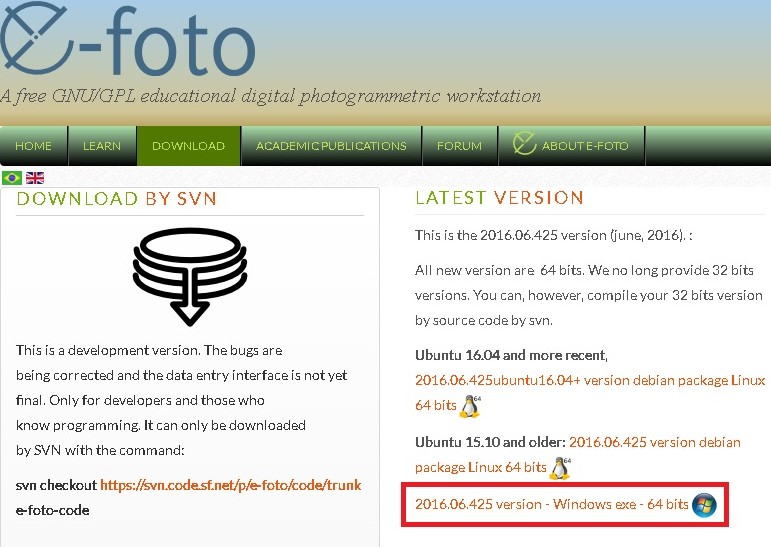
\includegraphics[width=8cm, center]{figuras/downmsi.jpg}
	\caption{Realizando download do instalador do E-foto} \label{fig:downmsi}
\end{figure}

\subsubsection{Passo 2 - Realizar a instalação}
Normalmente o arquivo baixado vai para a pasta Downloads do computador do usuário e para realizar a instalação basta dar um clique duplo nesse arquivo, clicar na opção Next, ler e aceitar os termos do contrato e clicar novamente em Next, no próximo passo o usuário deve escolher o caminho onde o E-foto será instalado e depois o usuário deve clicar em Install e a instalação será realizada automaticamente conforme a figura \ref{fig:installmsi}.
 
\begin{figure}[!ht]{17cm}
   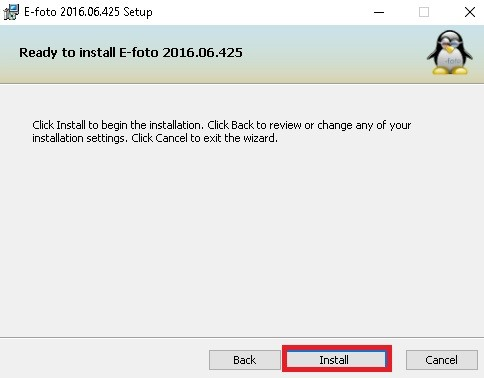
\includegraphics[width=8cm, center]{figuras/installmsi.jpg}
   \caption{Instalando E-foto através do instalador} \label{fig:installmsi}
\end{figure}
  
\subsubsection{Passo 3 - Executar o programa E-foto}
Após a instalação terminar, basta manter a opção launch E-foto e clicar na opção Finish, como mostra a figura \ref{fig:launch1} que o E-foto será executado, ou fechar o instalador e buscar o E-foto nos seus aplicativos instalados conforme a figura \ref{fig:launch2}. Neste formato o instalador do E-foto instalará tudo o que é necessário para o funcionamento sem a necessidade de configurações adicionais.
%detalhes, detalhes. Capture telas, coloque as imagens aqui. explique passo a passo. Ainda está muito genérico.

\begin{figure}[!ht]{17cm}
	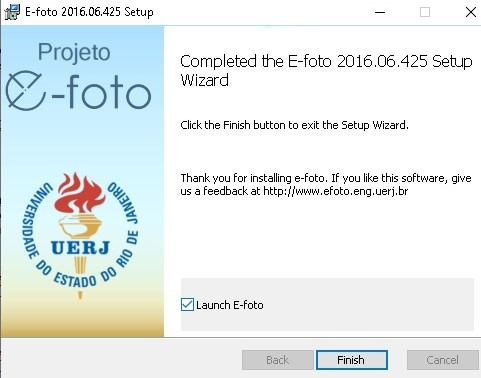
\includegraphics[width=8cm, center]{figuras/launch1.jpg}
	\caption{Executando o E-foto pelo instalador} \label{fig:launch1}
\end{figure}

\begin{figure}[!ht]{17cm}
	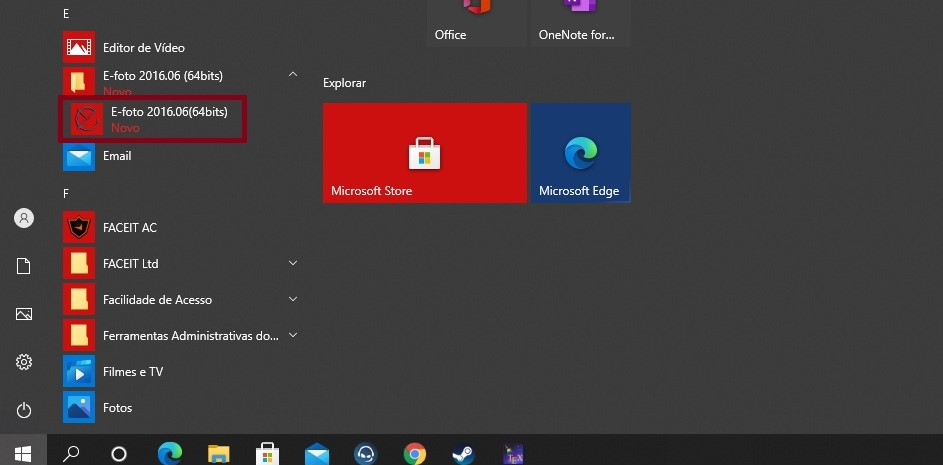
\includegraphics[width=8cm, center]{figuras/launch2.jpg}
	\caption{Buscando E-foto nos aplicativos} \label{fig:launch2}
\end{figure}



\subsection{Compilação do E-foto a partir dos fontes}
\subsection{Em Sistemas Linux}

\subsubsection{Passo 1 - Baixar código fonte}
Primeiramente, para realizar a instalação do software E-foto, o usuário deve fazer o download do seu código fonte e para isso é necessário a instalação do subversion, se já não estiver instalado. Para tal, o usuário deve abrir o terminal do seu sistema Linux, que pode ser feito digitando terminal na barra de busca ao apertar a tecla do Windows no seu teclado ou pelo atalho do teclado \texttt{ctrl + alt + T}. Com o terminal aberto, o usuário começará a instalação do SVN com os comandos: 
\begin{lstlisting}[language=bash]
	$ sudo apt update
	$ sudo apt install subversion
\end{lstlisting}

Com o SVN instalado e configurado, basta o usuário digitar no terminal o comando:
\begin{lstlisting}[language=bash]
 $ svn checkout https://svn.code.sf.net/p/e-foto/code
\end{lstlisting}

Com a utilização desse comando o download de todo o código fonte do software E-foto será feito automaticamente.  
    
\subsubsection{Passo 2 - Instalar pacotes necessários à compilação}  
Após a realização do download do código fonte do E-foto, o usuário deve ficar atento aos pacotes necessários em seu ambiente para que o software E-foto possa ser instalado e ter seu funcionamento sem erros. Para a instalação dos pacotes o usuário deve buscar abrir novamente o terminal. Os pacotes necessários para instalação do e-foto são:
\begin{itemize}
   	\item libgdal.dev
   	\item build-essential
   	\item libfontconfig1
   	\item mesa-common-dev
   	\item libx11-xcb-dev
   	\item libglu1-mesa-dev
\end{itemize}
Cada pacote deve ser instalado com respectivamente com os seguintes comandos:	
\begin{lstlisting}[language=bash]
	$ sudo apt install libgdal-dev
	$ sudo apt install build-essential
	$ sudo apt install libfontconfig1
	$ sudo apt install mesa-common-dev
	$ sudo apt install libx11-xcb-dev 
	$ sudo apt install libglu1-mesa-dev
\end{lstlisting}				
	
O pacote libgdal.dev é o contém as funcionalidades da GDAL, onde GDAL é uma biblioteca de tradução para formatos geoespaciais. O pacote libfontconfig1 contém uma biblioteca projetada para achar fontes no sistema e selecioná-las de acordo com os requisitos especificados pelas aplicações, e o usuário deve instalar o driver XCB e o OpenGl através dos pacotes mesa-common-dev, libx11-xcb-dev e libglu1-mesa-dev. 
    
\subsection{Passo 3 - Instalar os pacotes de instalação do Qt 5}   
A instalação do Qt 5 via terminal deve ser feita através dos seguintes pacotes:
\begin{itemize}
	\item qt5-default
	\item qt5-qmake
\end{itemize}   
Esses pacotes devem ser instalados através dos seguintes comandos do terminal:
\begin{lstlisting}[language=bash]
	$ sudo apt install qt5-default
	$ sudo apt install -y qt5-qmake
\end{lstlisting}	
    
Após esses procedimentos o usuário ja terá um ambiente de compilação pronto para a instalação do E-foto, assim como o plataforma em que o mesmo foi desenvolvido.
    
\subsection{Passo 4 - Compilar e executar o software E-foto}
Para compilar e executar o código do E-foto via terminal, após a realização de todos os passos necessários, o usuário deve utilizar os seguintes comandos no terminal:
\begin{lstlisting}[language=bash]
   	$ cd diretório/
   	$ qmake e-foto.pro
   	$ make
   	$ ./build/bin/e-foto
\end{lstlisting}
   
O comando cd diretório/ servirá para o usuário percorrer o caminho até o diretório onde está o arquivo e-foto.pro (atualmente code/branches/e-foto-trunk-candidate), depois o qmake e o make irão realizar a compilação e gerar o executável do E-foto. Por fim o último comando irá executar o software E-foto.

\subsection{Em Sistemas Windows}

\subsubsection{Passo 1 - Baixar código fonte}
 Para começara instalação do E-foto em sistemas Windows, o usuário deve realizar o download do código fonte do E-foto e para isso o melhor caminho é ulilizar o subversion, que no Windows pode ser feito através de um programa chamado TortoiseSVN que pode ser baixado gratuitamente por esse link https://tortoisesvn.net/downloads.html na opção mostrada na figura \ref{fig:tortoise}, após a instalação do TortoiseSVN, o usuário deve buscar no programa a opção de SVN Checkout, que pode ser encontrada ao clicar o botão direito do mouse na área de trabalho conforme é mostrado na figura \ref{fig:checkout} e no espaço para colar uma URL (primeira opção disponível) colocar https://svn.code.sf.net/p/e-foto/code como é visto na figura \ref{fig:url}, que deve gerar o download de todo o código fonte do E-foto.
 
 \begin{figure}[!ht]{17cm}
 	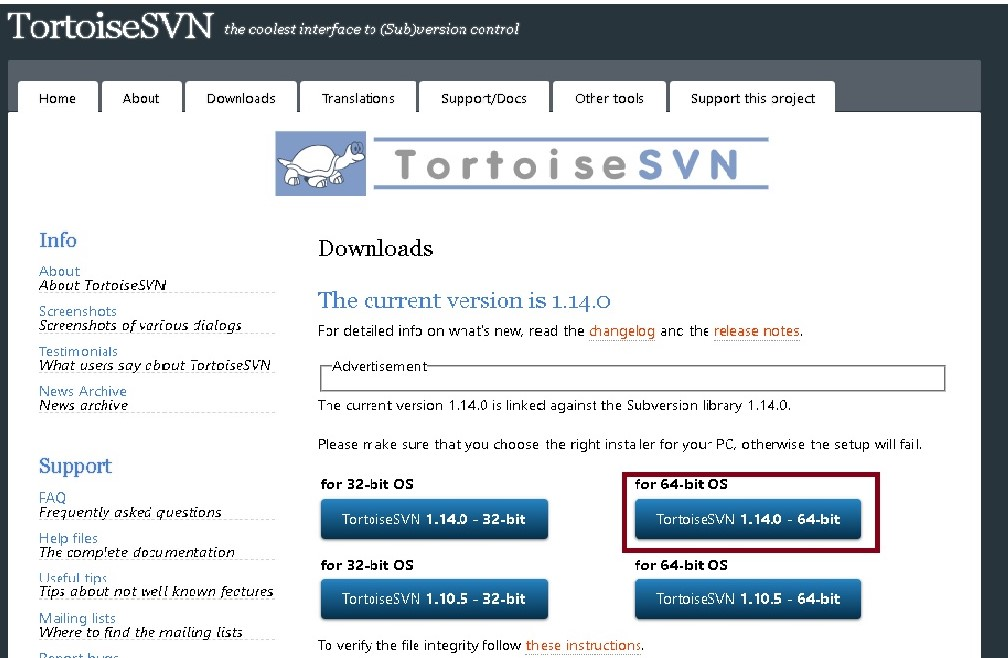
\includegraphics[width=8cm, center]{figuras/tortoise.jpg}
 	\caption{Download do TortoiseSVN} \label{fig:tortoise}
 \end{figure}

\begin{figure}[!ht]{17cm}
	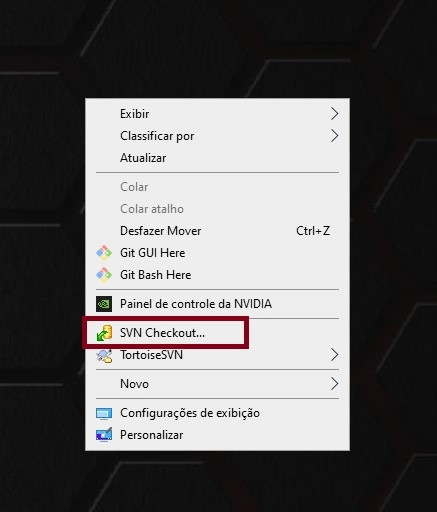
\includegraphics[width=8cm, center]{figuras/checkout.jpg}
	\caption{Buscando a opção de checkout} \label{fig:checkout}
\end{figure}

\begin{figure}[!ht]{17cm}
	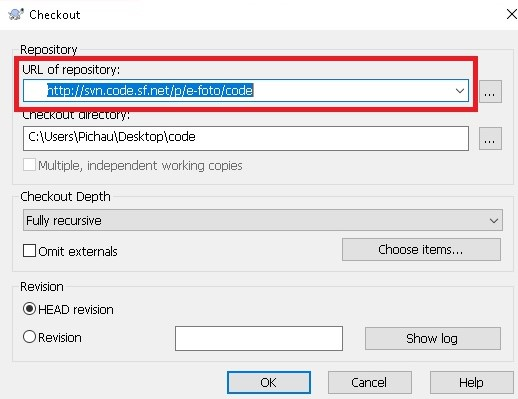
\includegraphics[width=8cm, center]{figuras/url.jpg}
	\caption{Realizando o download com a URL} \label{fig:url}
\end{figure}
 
\subsubsection{Passo 2 - Download dos pacotes binários da Gdal no Windows} 
 O próximo passo é o download dos pacotes binários do Gdal no Windows que pode ser realizado através desse link https://repo.msys2.org/distrib/x86\_64/msys2-x86\_64-20200720.exe, que realizará o download do MSYS, após a conclusão do download e da instalação do MSYS (que deve ser feita no drive C, que normalmente é o default) o usuário deve executar mSYS, o que vai abrir o terminal do próprio MSYS que contém uma versão portada do gerenciador de pacotes Pacman conforme pode ser visto na figura \ref{fig:terminalgdal}, nessa última versão do Pacman deve ser digitado no terminal o comando:
 
 \begin{figure}[!ht]{17cm}
 	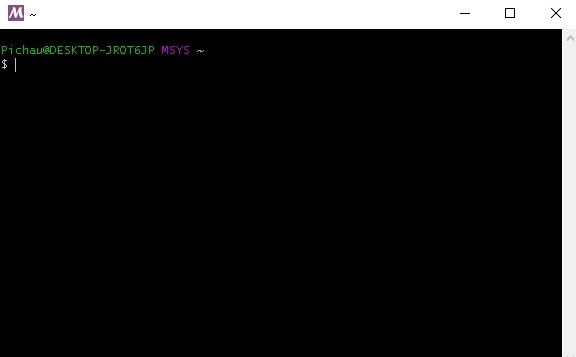
\includegraphics[width=8cm, center]{figuras/terminalgdal.jpg}
 	\caption{Terminal MSYS} \label{fig:terminalgdal}
 \end{figure}
 
 \begin{lstlisting}[language=bash]
 	$ pacman -Syuu
 \end{lstlisting}

 Esse comando irá gerar uma série de instruções a serem seguidas até que o usuário possa repetir o comando e receber a mensagem de que nada necessita ser atualizado. Com o ambiente atualizado, o usuário deve digitar o seguinte comando:
  \begin{lstlisting}[language=bash]
 	$ pacman -S mingw64/mingw-w64-x86\_64-gdal
 	$ gdalinfo --version
 \end{lstlisting}

 Esses comandos que realizarão finalmente o download e instalação dos pacotes binários da GDAL e dirão qual versão que foi instalado, respectivamente. 
 
 \subsubsection{Passo 3 - Baixar e configurar o Qt 5 e o Qt Creator}
 Nessa etapa o usuário deve realizar o download do Qt 5 e do Qtcreator no website https://www.qt.io/download como mostrado na figura \ref{fig:downqt} , deixando claro que na parte da instalação deve ser escolhido para instalar apenas as opções do mingw 64-bits, e o Qt 5 referente a esse sistema que é visto na figura \ref{fig:qtinstallconfig}. Com os arquivos do código fonte do E-foto disponíveis o usuário deve procurar no caminho e-foto-code/branches/e-foto-trunk-candidate por um arquivo chamado e-foto.pro mostrado na figura \ref{fig:openpro}. Quando abrir o projeto no Qtcreator será necessário configurar o que deverá ser usado, começando pela escolha do kit que será usado que devem ser os mesmos escolhidos na instalação do Qt 5, ou seja, o mingw 64-bits e a versão do Qt referente a esse sistema como mostra a figura \ref{fig:qtkit}. Após o projeto estar aberto, o usuário deve ir na guia project e desmarcar a opção shadow build, e depois procurar na aba build a opção build E-foto, quando acabar a compilação é só clicar na opção Run que também pode ser encontrado na aba build e o E-foto vai abrir pronto para o uso como estão assinalados na figura \ref{fig:projectbuild}.
 %coloque capturas de tela aqui. Aliás, como o processo é gráfico, sempre use capturas de telas e não simplesmente texto.
  \begin{figure}[!ht]{17cm}
 	
\includegraphics[width=8cm, center]{figuras/downqt.jpg}
 	\caption{Download do Qt 5 pelo website} \label{fig:downqt}
 \end{figure}

 \begin{figure}[!ht]{17cm}
	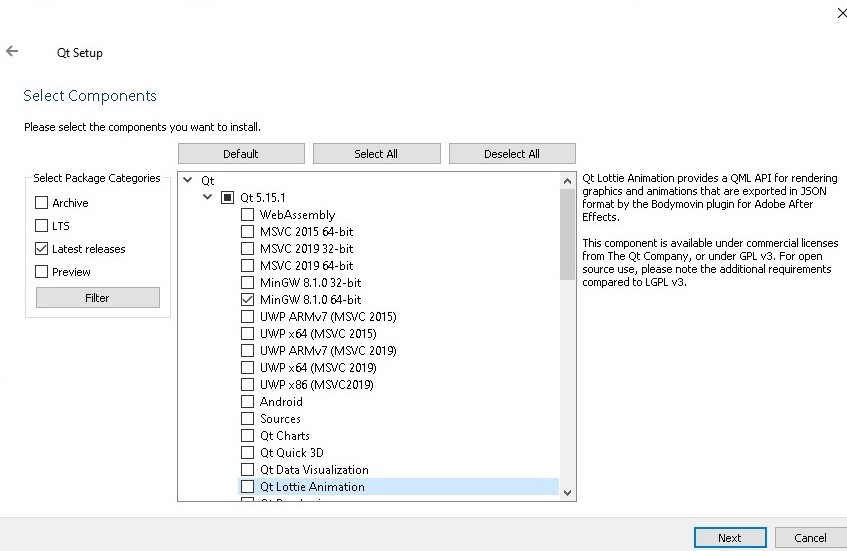
\includegraphics[width=8cm, center]{figuras/qtinstallconfig.jpg}
	\caption{configuração da  instalação do Qt 5} \label{fig:qtinstallconfig}
\end{figure}

 \begin{figure}[!ht]{17cm}
	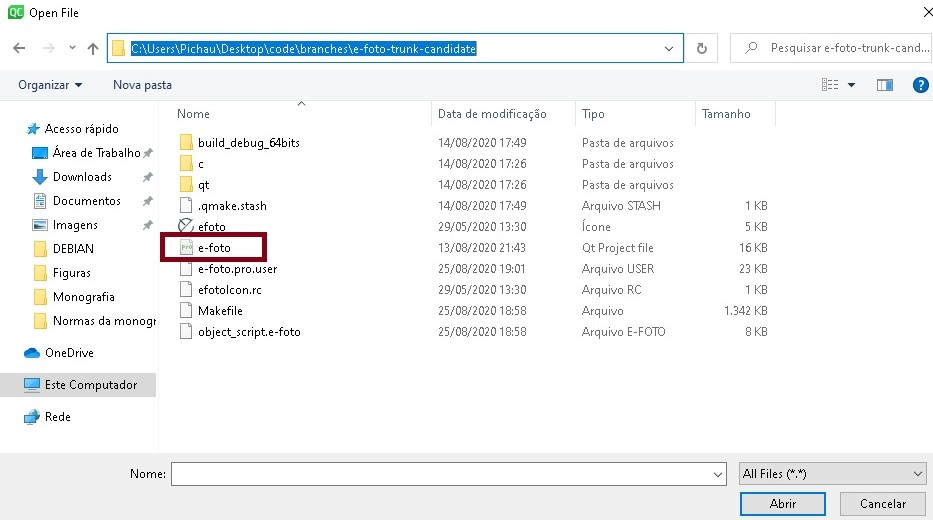
\includegraphics[width=8cm, center]{figuras/openpro.jpg}
	\caption{Caminho do arquivo do projeto E-foto} \label{fig:openpro}
\end{figure}

 \begin{figure}[!ht]{17cm}
	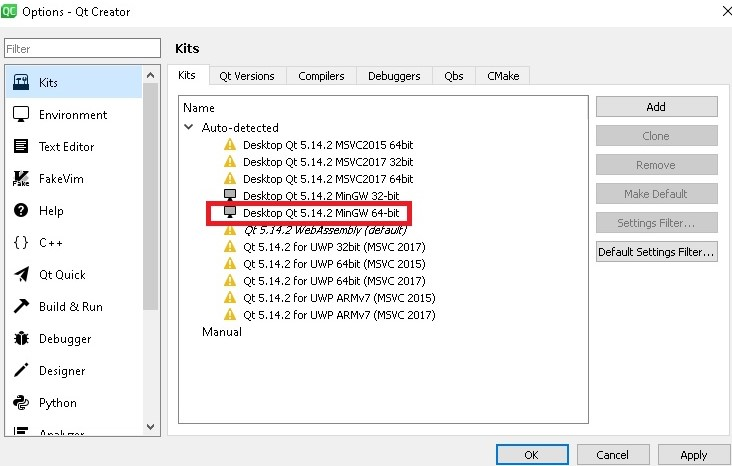
\includegraphics[width=8cm, center]{figuras/qtkit.jpg}
	\caption{Configuração do kit} \label{fig:qtkit}
\end{figure}

 \begin{figure}[!ht]{17cm}
	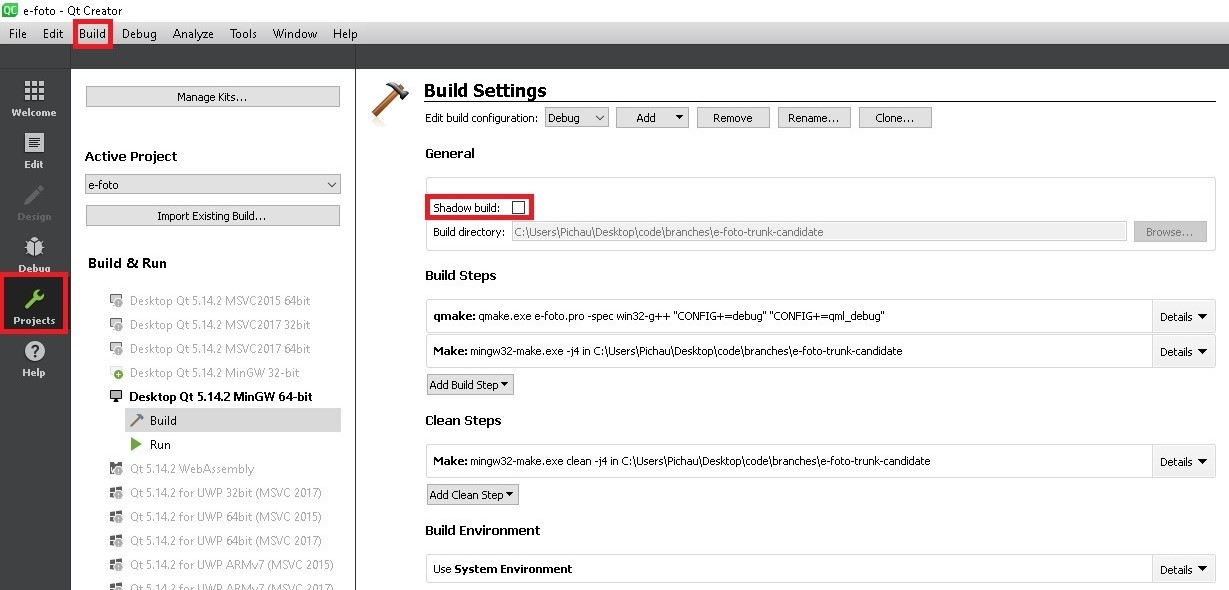
\includegraphics[width=8cm, center]{figuras/projectbuild.jpg}
	\caption{Locais buscados para a compilação} \label{fig:projectbuild}
\end{figure}
 